\section{Results}\label{sec:results}

I don't think I even need a section for this...
Just reference it in the Implementation section and the Conclusions section.

Talk about losses?
Here are the confusion matrices.
Here are some examples of images, pertebations, and resulting perturbed images.
I could also find the n closest signatures to a signature and see what that looks like...
Also try pertebations on swapped networks!
Also, try to perturb non-matching signatures and even random noise...

Also plot distances (genuine and impostor and adversarial impostor) for SigNet128 to see if they are actually Gaussian...

I could also dot product normalized gradients of successive pertebations to see how similar the directions are...

Here's a table of the accuracy (true/false positive/negative matix).
% todo: compute matrix...

\begin{table*}[t]
    \centering
    \begin{tabular}{|c | c >{\em}c | >{\em}c c | >{\bfseries}c | >{\em}c c >{\bfseries}c|}
    % \begin{tabular}{|m{2.5cm} | m{1cm} | m{1cm} | m{1cm} | m{1cm} | m{1cm} | m{1cm} | m{1cm} | m{1cm}|}
        \hline
        % lvd & tp & fn & fp & tn & acc & fpi & tni & acci\\ [0.1ex]
        % Dimensionality & true positive & false negative & false positive & true negative & accuracy & false positive imp & true negative imp & accuracy imp\\ [0.1ex]
        \multirow{3}{*}{Dimensionality} & \multicolumn{5}{c|}{Normal} & \multicolumn{3}{c|}{Adversarial}\\
        \hline
        & \multicolumn{2}{c|}{Positive} & \multicolumn{2}{c|}{Negative} & \multirow{2}{*}{Accuracy} & Positive & Negative & \multirow{2}{*}{Accuracy}\\
        % \hline
        & True & False & False & True & & False & True & \\
        \hline
        64 & 1144 & 4 & 236 & 1376 & 91.30 & 450 & 930 & 75.14\\
        128 & 1044 & 224 & 336 & 1156 & 79.71 & 1211 & 169 & 43.95\\
        256 & 729 & 88 & 651 & 1292 & 73.22 & 377 & 1003 & 62.75\\ [0.1ex]
        \hline
    \end{tabular}
    \caption{Comparison of Accuracy using Latent Vector Sizes after 5 Epochs}
    \label{table:1}
\end{table*}

\begin{table*}[t]
    \centering
    \begin{tabular}{|c | c >{\em}c | >{\em}c c | >{\bfseries}c | >{\em}c c >{\bfseries}c|}
    % \begin{tabular}{|m{2.5cm} | m{1cm} | m{1cm} | m{1cm} | m{1cm} | m{1cm} | m{1cm} | m{1cm} | m{1cm}|}
        \hline
        % lvd & tp & fn & fp & tn & acc & fpi & tni & acci\\ [0.1ex]
        % Dimensionality & true positive & false negative & false positive & true negative & accuracy & false positive imp & true negative imp & accuracy imp\\ [0.1ex]
        \multirow{3}{*}{Dimensionality} & \multicolumn{5}{c|}{Normal} & \multicolumn{3}{c|}{Adversarial}\\
        \hline
        & \multicolumn{2}{c|}{Positive} & \multicolumn{2}{c|}{Negative} & \multirow{2}{*}{Accuracy} & Positive & Negative & \multirow{2}{*}{Accuracy}\\
        % \hline
        & True & False & False & True & & False & True & \\
        \hline
        64 & 1347 & 0 & 33 & 1380 & 98.80 & 39 & 1341 & 97.39\\
        128 & 1366 & 0 & 14 & 1380 & 99.49 & 91 & 1289 & 96.20\\
        256 & 1353 & 0 & 27 & 1380 & 99.02 & 89 & 1291 & 95.80\\ [0.1ex]
        \hline
    \end{tabular}
    \caption{Comparison of Accuracy using Latent Vector Sizes after 20 epochs}
    \label{table:2}
\end{table*}



As mentioned in section \ref{sec:cedar_flaw}, there is at least one significant difference between the genuine and forge images in the CEDAR dataset.
Since CNNs are very powerful and should be able to pick up on this difference very easily, the CEDAR dataset is not a good test of an architecture's ability to understand or verfiy handwritten signatures.

\begin{figure}[h]
    \begin{center}
        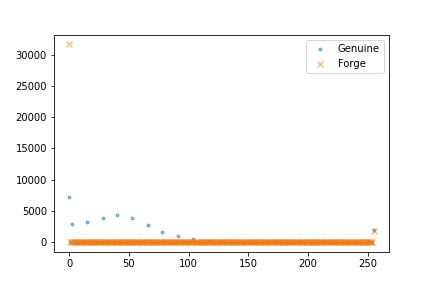
\includegraphics[width=0.8\linewidth]{mean_hist.png}
    \end{center}
    \caption{Histogram of Means of Binned Pixel Values}
    \label{fig:hist_pixel_values}
\end{figure}

Here's a genuine and a forge and we apply various epsilon values and also repeat...
    There are diminising returns on continually nudging a forge.

Here's how well we trick SigNet...

Here's the same thing with 2 genuines of different signatures.

Here's the same thing with 2 genuines of the same signature.


If I need more content, I could graph the training loss and talk about how it stabilzes.

the accuracy after \_ amount of training was 72% accuracy
It would take too long to get 100% accuracy

The validation loss was higher than the training loss even on the 1st epoch of training.
I believe this is because the images in the datapoints (image pairs with labels) have been seen before...


random noise can score well...

-------------------------------------------------

There are pure 0s in the forge, but not the original...
what if I add a bit of random noise to the forge?

I wonder if making the pixels boolean would help or hurt signet/advarsary...





WAT
    scaling the input to the net doesn't seem to change its output (latent) vector
    It that because it is doing some sort of normalization??
